% Название разделов -- все прописные
\section{АКТУАЛЬНОСТЬ ТЕМЫ}
%ссылки на рисунки по человечески сделать
Говоря о применении ОДУ легче найти области, где они не применяются.
Их используют в физике для моделирования процессов, начиная от баллистики и заканчивая перемещением
по твёрдой поверхности, биологии для прогнозирования динамики биологических популяций, тонких технологических процессах и так далее.
На рисунке \ref{fig:actuality} показаны области использования ОДУ.
Прогнозировать те или иные процессы можно как при помощи натурных экспериментов, так и с помощью численного моделирования.

\begin{figure}
    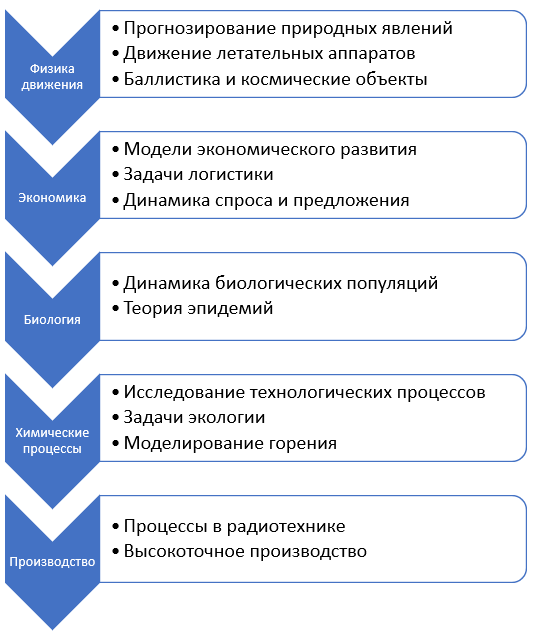
\includegraphics[width=10cm]{2-00-actuality}
    \caption{Области применения ОДУ}
    \label{fig:actuality}
\end{figure}

Для численного моделирования тех или иных процессов нужно использовать специализированные программы и библиотеки, которых на
сегодняшний день предоставлено большое количество, однако все они имеют свои ограничения и недостатки.